% This text is proprietary.
% It's a part of presentation made by myself.
% It may not used commercial.
% The noncommercial use such as private and study is free
% Sep. 2005 
% Author: Sascha Frank 
% University Freiburg 
% www.informatik.uni-freiburg.de/~frank/
% additional use of \usepackage{beamerthemesplit}
\documentclass{beamer}
\usepackage[utf8]{inputenc}
\usepackage[T2A]{fontenc} % кодировка шрифта
\usepackage[english,russian]{babel} % язык документа
\usepackage{beamerthemesplit}
\usepackage{graphicx}

\theoremstyle{plain}
\newtheorem{thm}{Теорема}[section]

\usepackage{beamerthemesplit} % new 
\begin{document}
\title{Компьютерная игра "Pchellout"} 
\author{Васильев Павел, Иудинов Михаил, Евтушенко Дмитрий}


 
\date{2 июня 2023 г.} 

\frame{\titlepage}

\section{Описание} 
\subsection{О чём игра}
\frame{ \frametitle{О чём игра}
Жанр: кликер-выживалка.

Игра про пчеловодство. Игрок имеет в своём владении улей с пчёлами и поляной с цветами. Игра заключается в том, чтобы спасти улей от нападения вражеских пчёл.

\begin{columns}
        \begin{column}{0.5\textwidth}
            \centering
            
\includegraphics[width=2cm]{images/bee.png}
        \end{column}

        \begin{column}{0.5\textwidth}
            \centering
            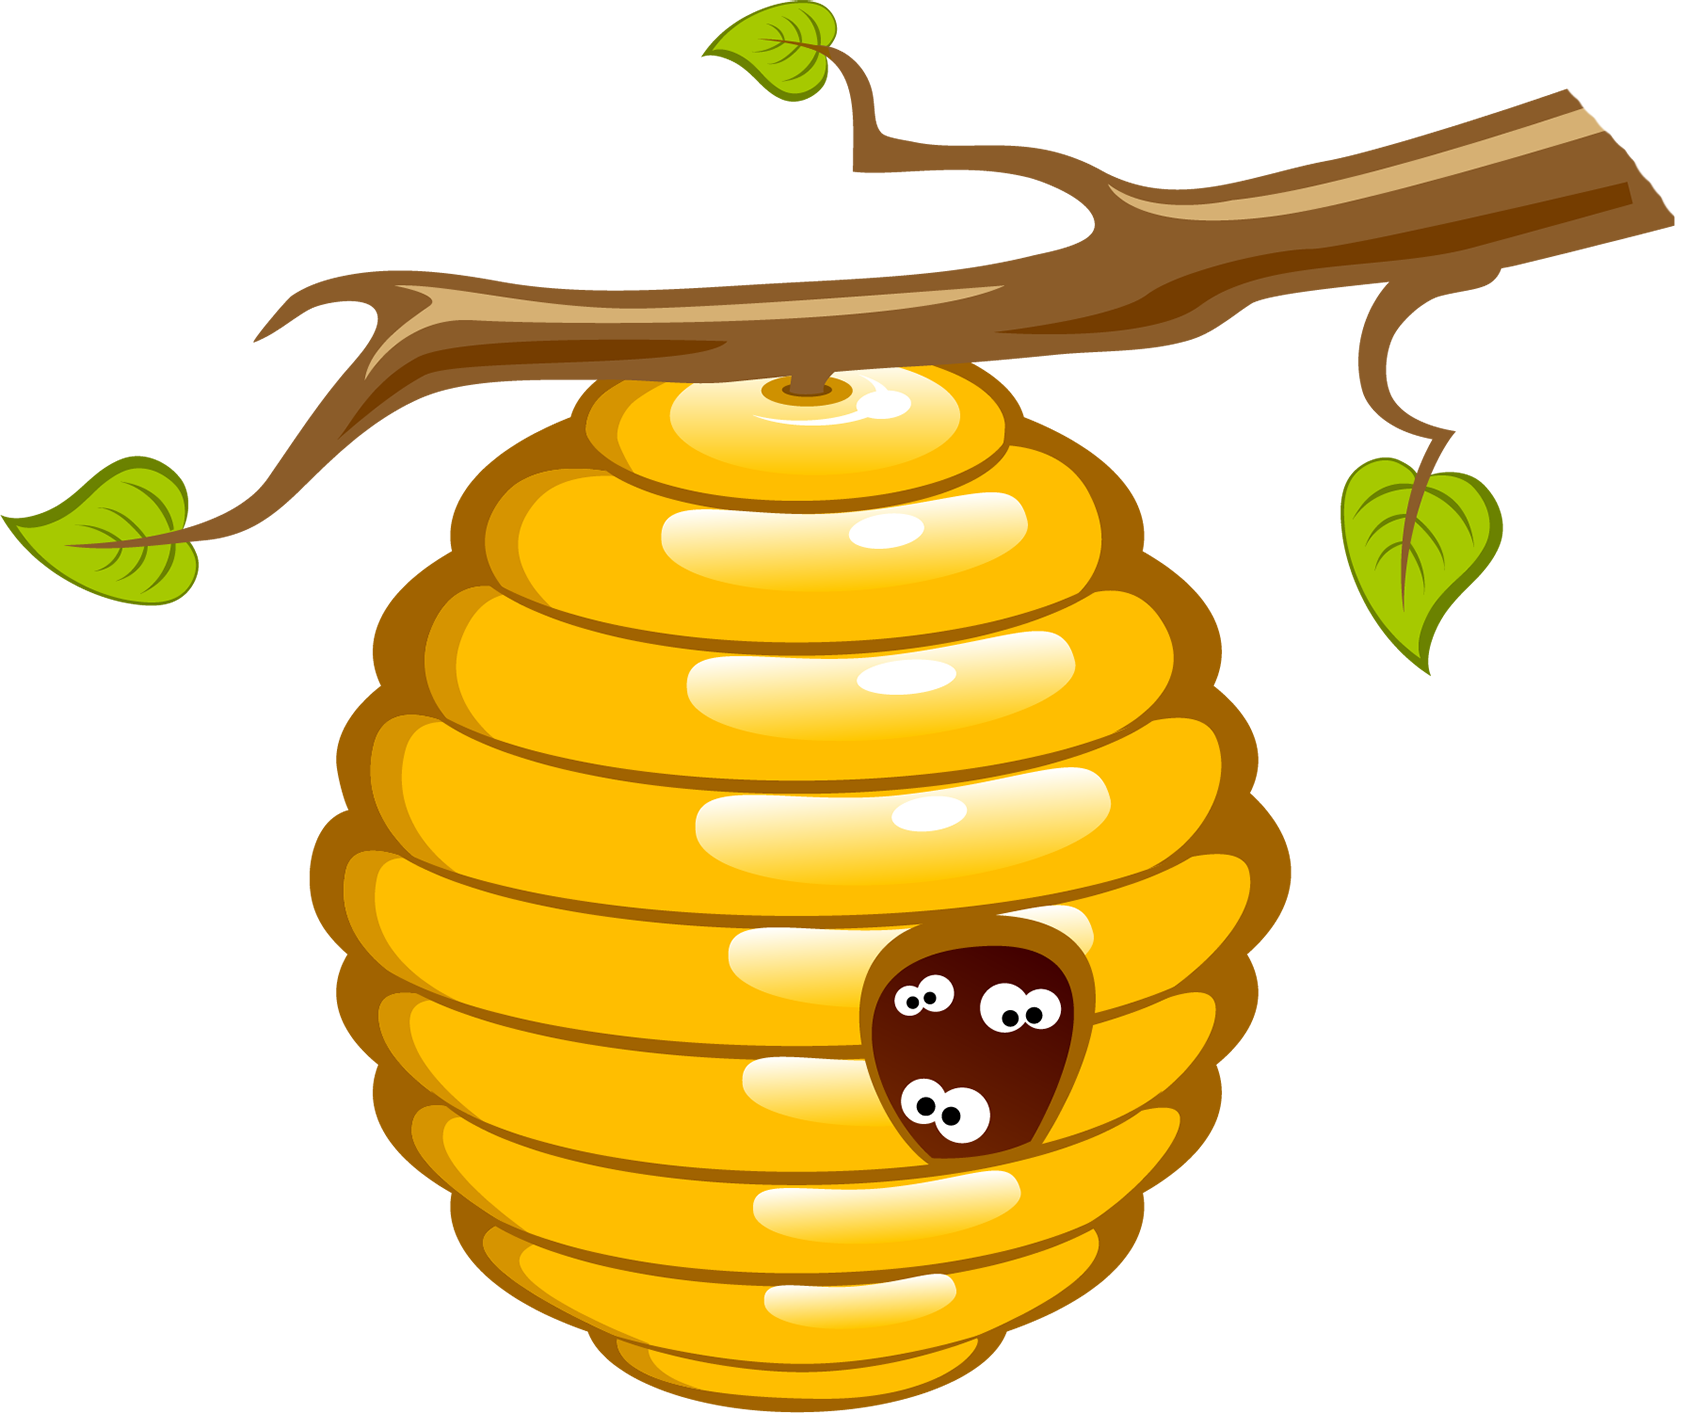
\includegraphics[width=4cm]{images/Hive.png}
        \end{column}
\end{columns}
}

\subsection{Референсы}
\frame{\frametitle{Референсы}

	\begin{columns}
        \begin{column}{0.3\textwidth}
            \centering
            
\includegraphics[width=3cm]{images/Clash_of_Clans.png}
        \end{column}

        \begin{column}{0.3\textwidth}
            \centering
            
\includegraphics[width=3cm]{images/Cookie_Clicker.png}
        \end{column}
        
        \begin{column}{0.3\textwidth}
            \centering
            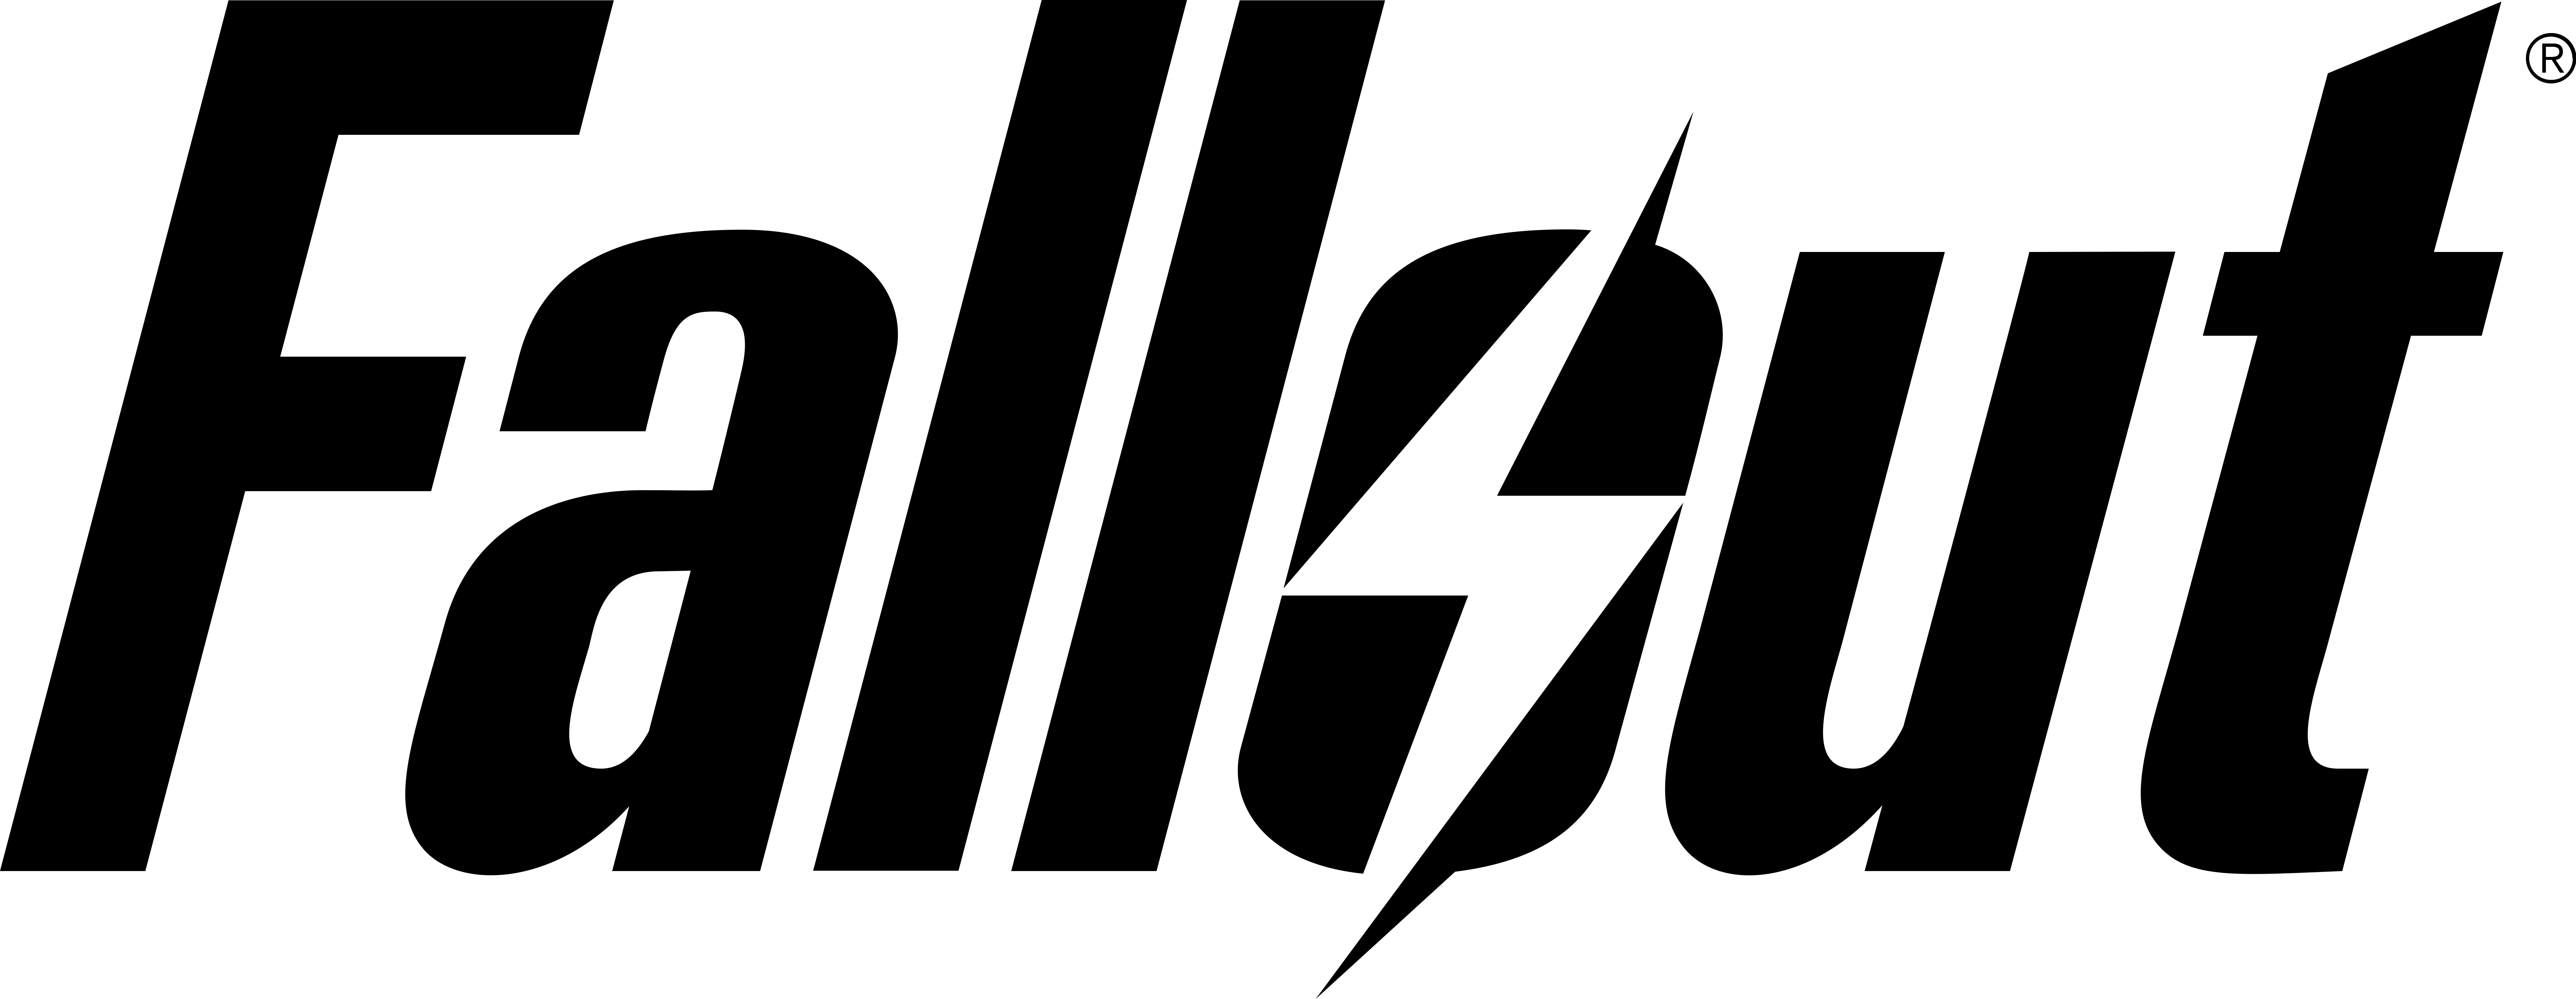
\includegraphics[width=3cm]{images/Fallout.png}
        \end{column}
    \end{columns}
	
}

\subsection{Геймплей и цели}
\frame{
\frametitle{Геймплей и цели}
Геймплей:
\begin{itemize}
\item есть главное строение - улей, который нужно оберегать
\item улей защищает пушка, которой управляет игрок
\item также есть кнопки для выпуска пчёл-защитников и сброса бомбы.
\item есть кнопка для спавна сборщиков мёда. Они нужны для переноса мёда от цветов (которые можно садить на поляну) в улей
\end{itemize}

\textit{Цель: защитить улей от вражеских пчёл, уничтожить босса и максимизировать количество собранного мёда}

}


\subsection{Скриншоты игры}
\frame{\frametitle{Скриншоты игры}
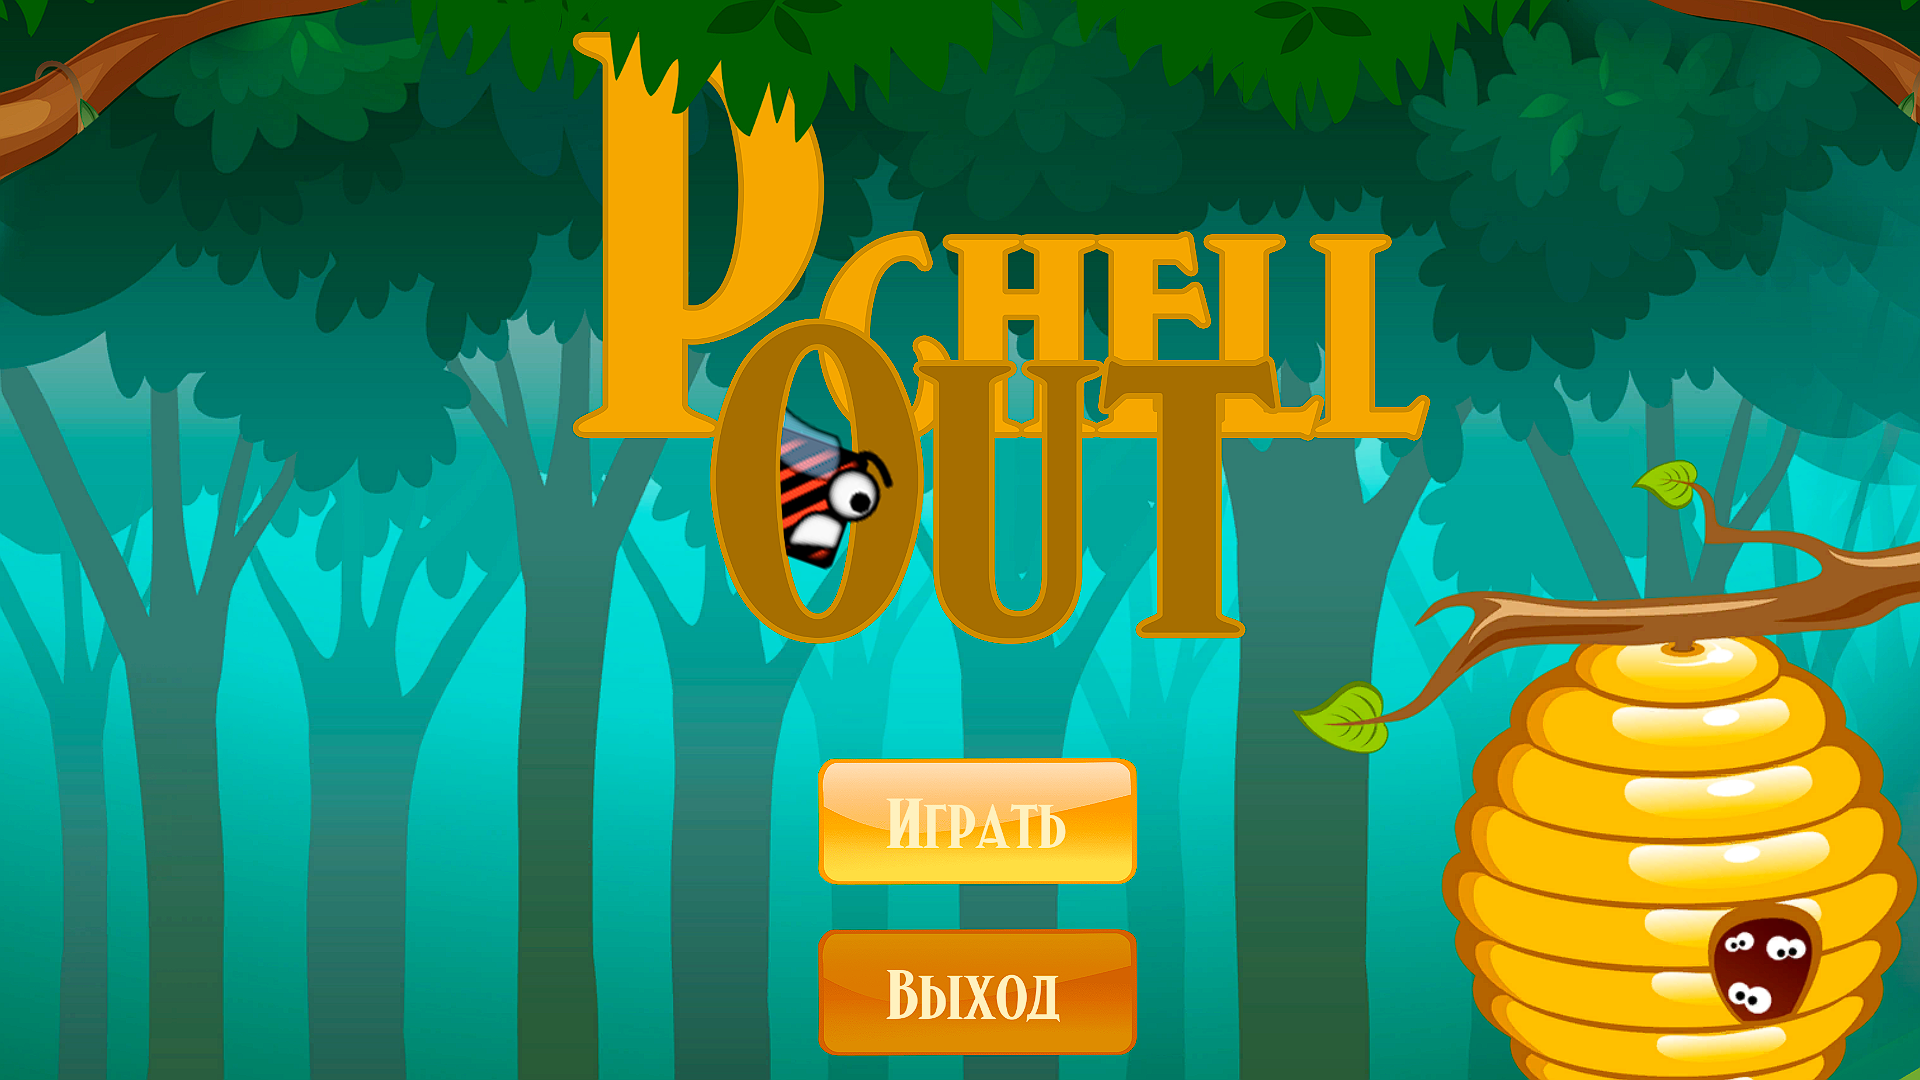
\includegraphics[width=11cm]{images/screen1.png}
}

\frame{\frametitle{Скриншоты игры}
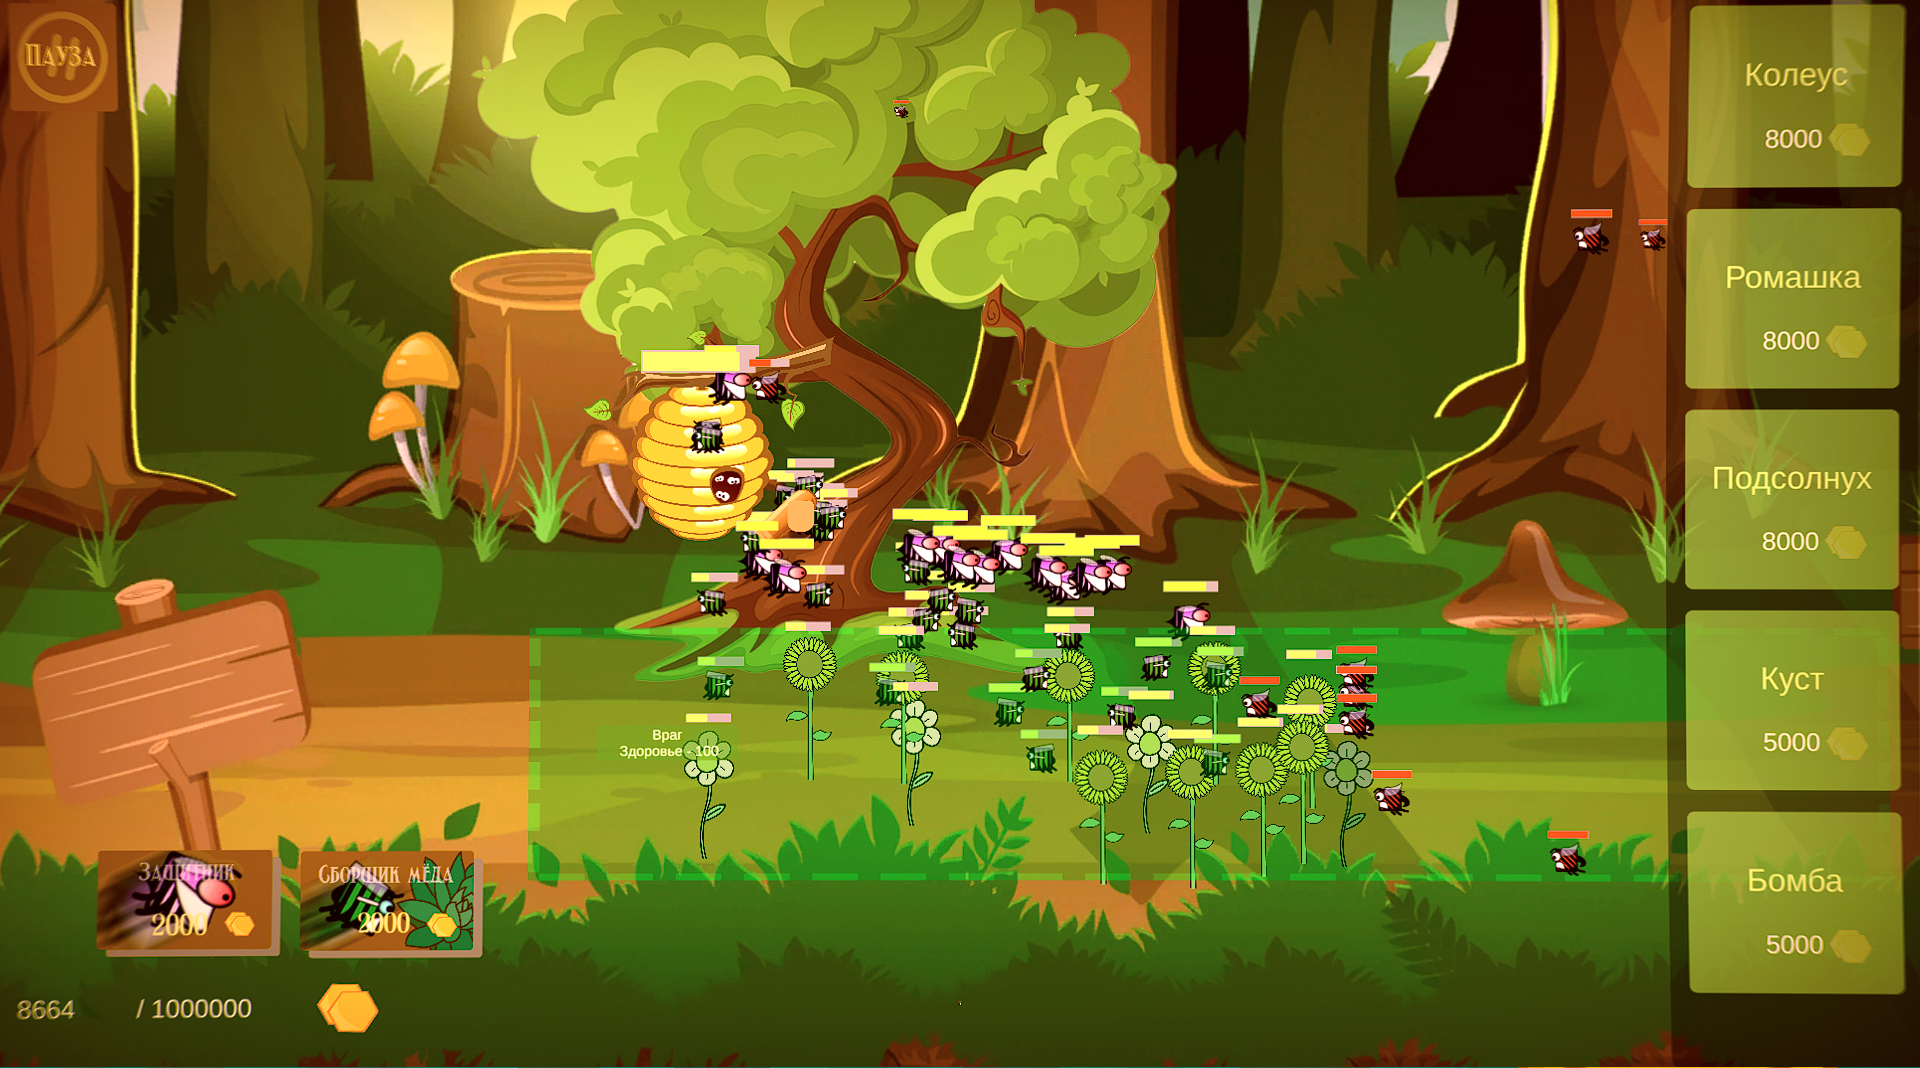
\includegraphics[width=11cm]{images/screen2.png}
}

\frame{\frametitle{Скриншоты игры}
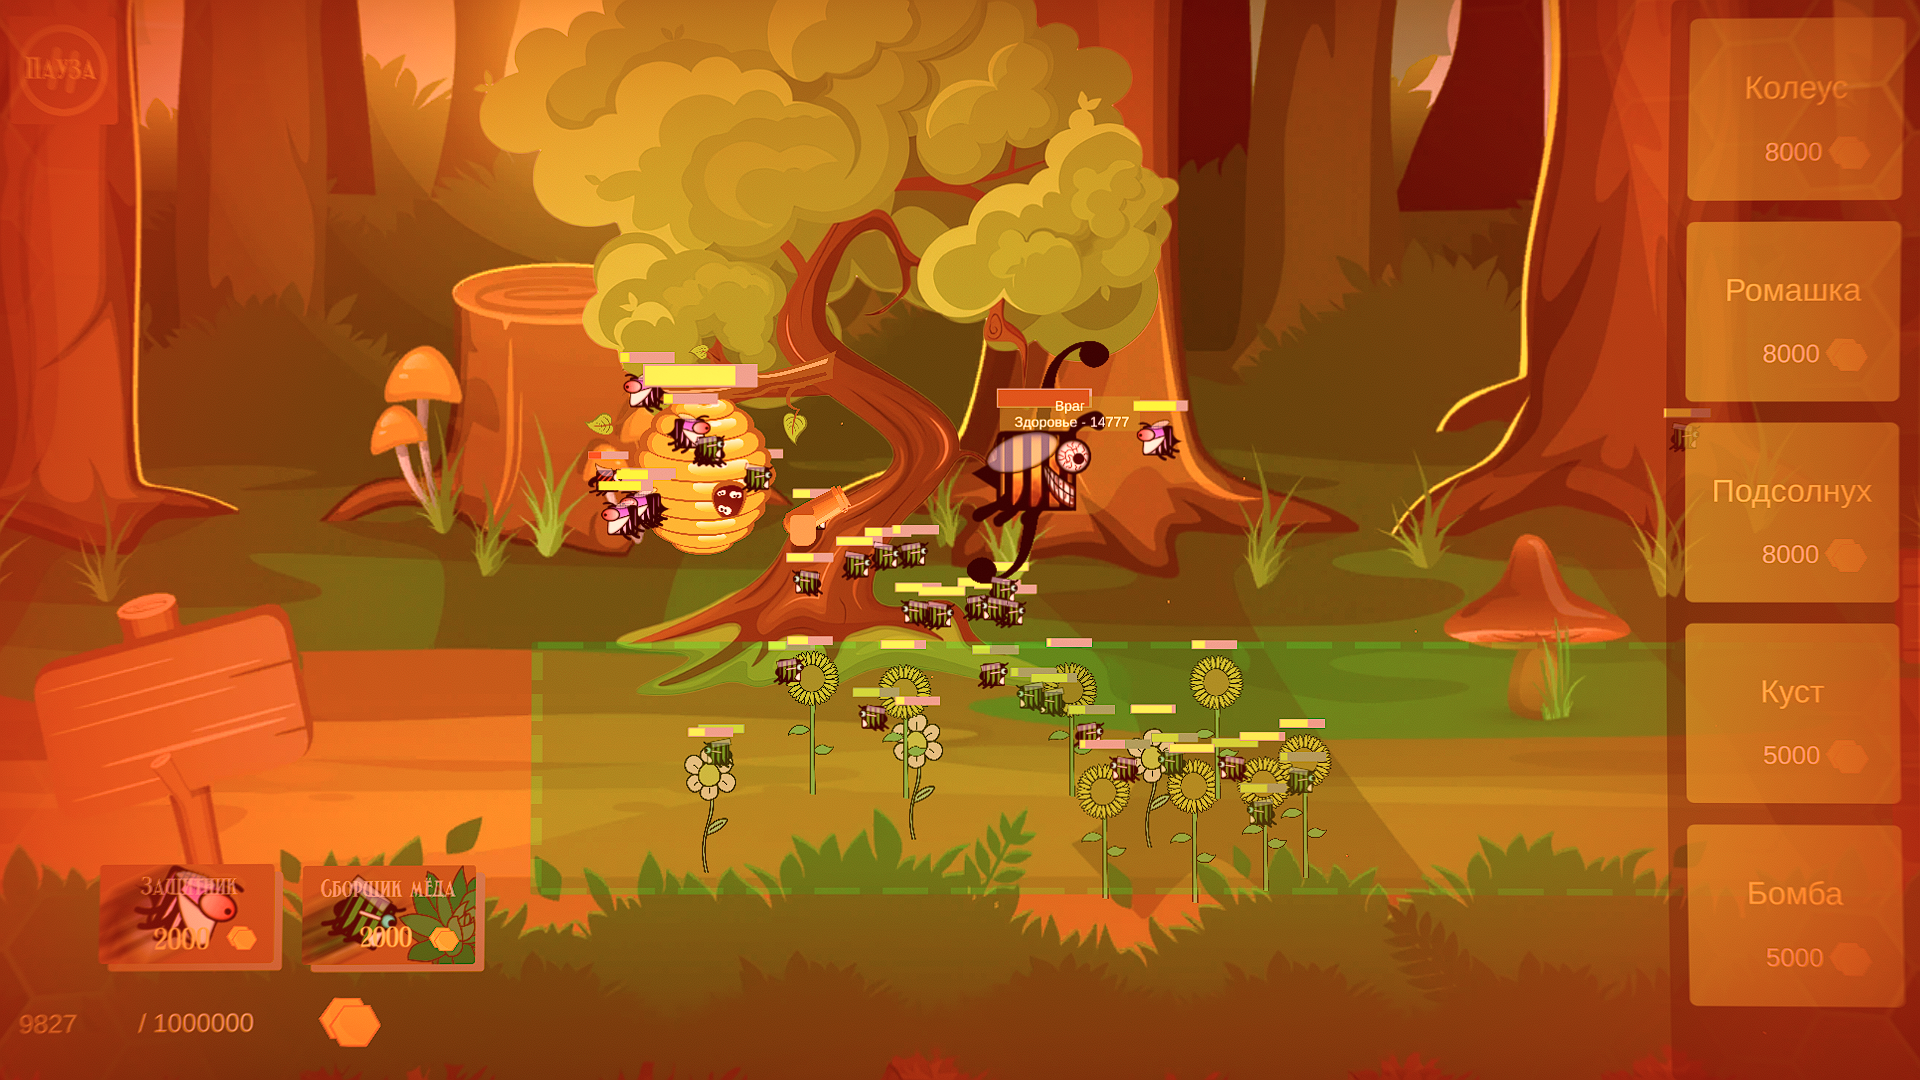
\includegraphics[width=11cm]{images/screen3.png}
}

\subsection{Роли в команде}
\frame{\frametitle{Павел Васильев}
Геймдизайнер, программист

\includegraphics[width=4cm]{images/pv.png}
}

\frame{\frametitle{Михаил Иудинов}
Разработчик UI, геймдизайнер
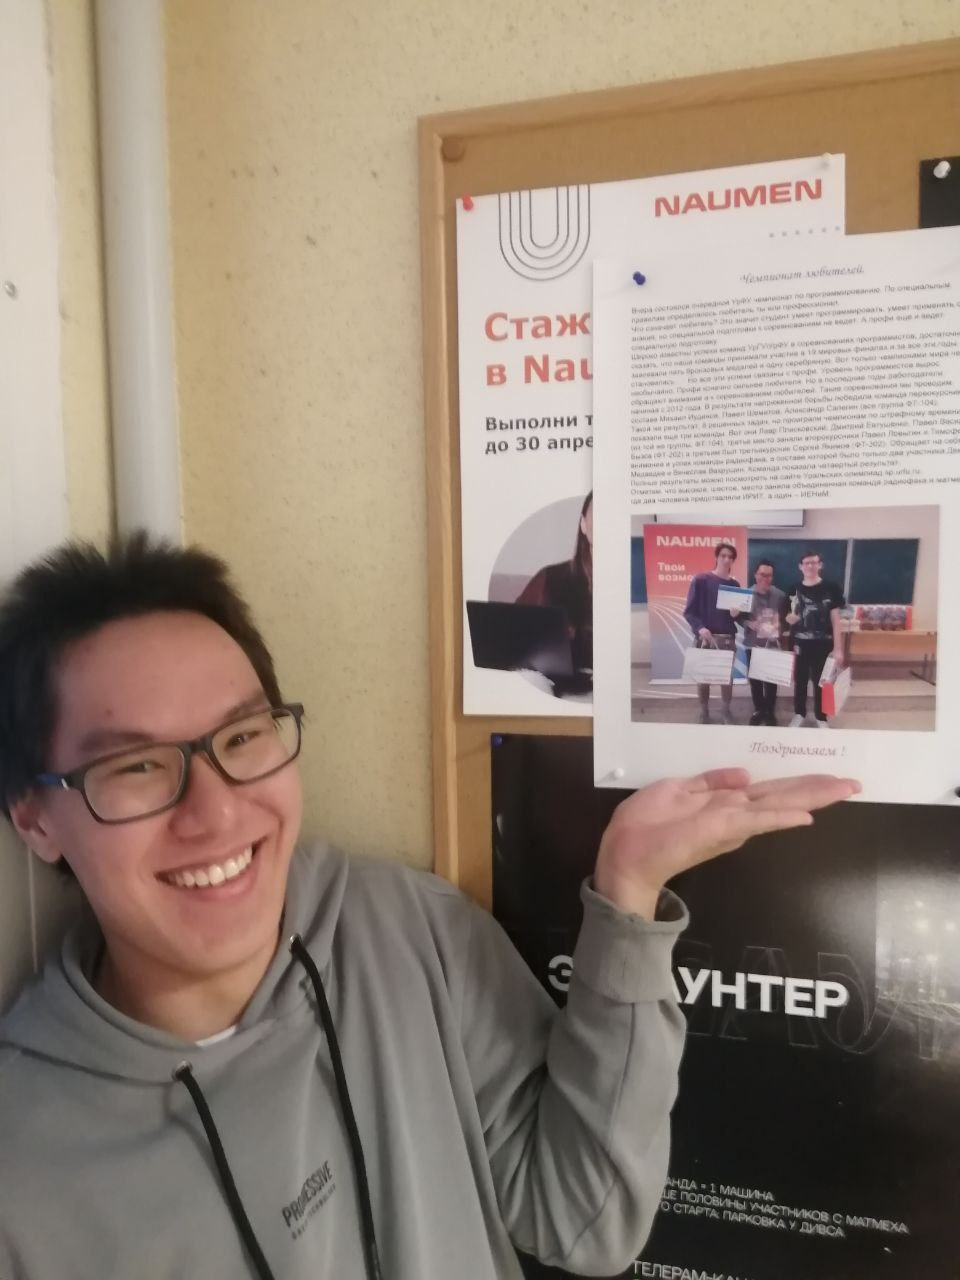
\includegraphics[width=4cm]{images/mi.jpg}
}

\frame{\frametitle{Дмитрий Евтушенко}
Звукорежиссёр, тестировщик, идейный вдохновитель
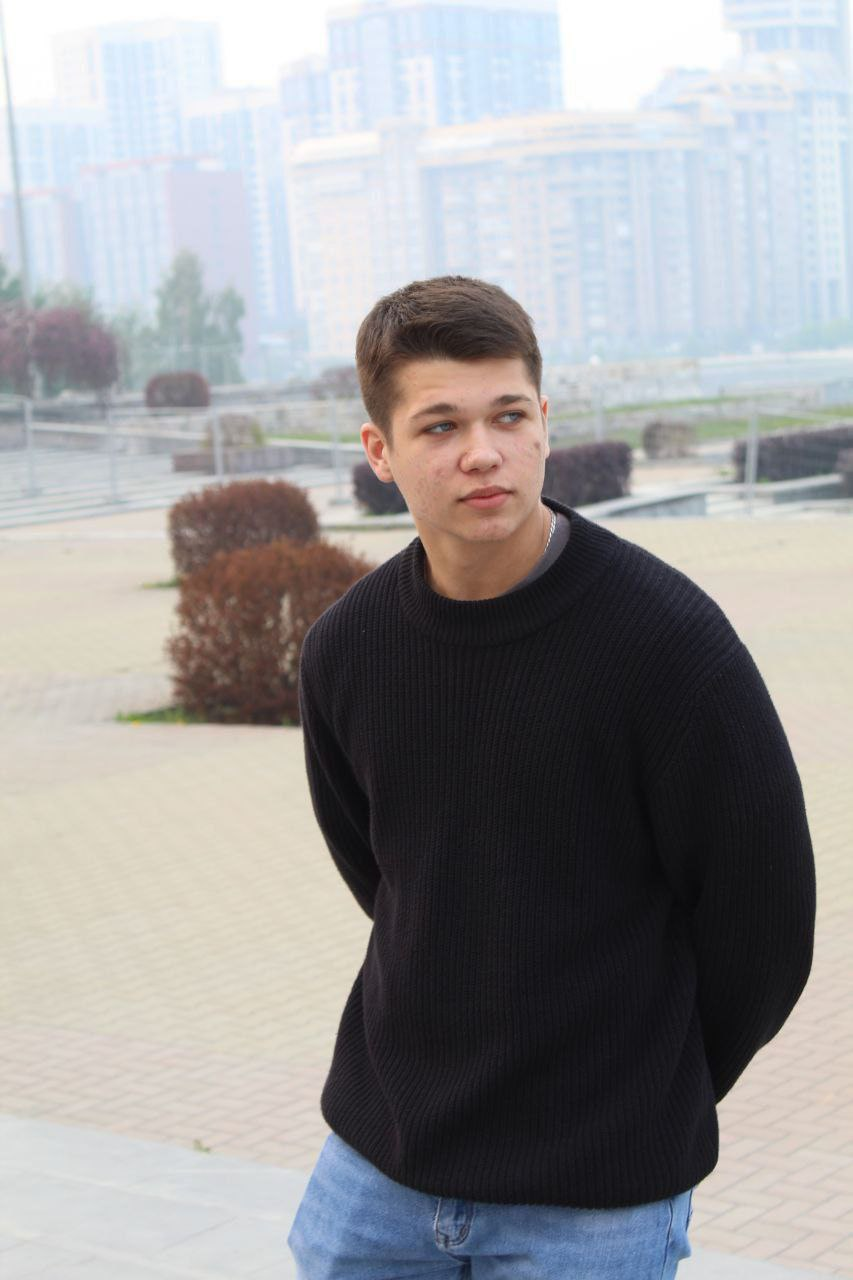
\includegraphics[width=4cm]{images/de.jpg}
}

\frame{
    \frametitle{Вопросы?}
    
    \begin{thm}
        Наша оценка по ОП - 5
    \end{thm}
    
    \begin{proof}
        Докажем от противного: пусть оценка не 5. Приходим к противоречию.
        \qedhere
    \end{proof}
}
\end{document}
